\documentclass[conference,letterpaper,10pt]{IEEEtran}

\usepackage[T1]{fontenc}
\usepackage[utf8]{inputenc}
\usepackage[english,spanish,es-tabla,es-noshorthands,es-nodecimaldot]{babel}
\usepackage{microtype}
\usepackage{amsmath,amssymb}
\usepackage{graphicx}
\usepackage{booktabs,array,tabularx,multirow}
\usepackage{xcolor}
\usepackage{cite}
\usepackage{xurl}
\usepackage{balance}
\setcounter{topnumber}{4}\setcounter{bottomnumber}{3}\setcounter{totalnumber}{6}\setcounter{dbltopnumber}{3}
\renewcommand{\topfraction}{0.96}\renewcommand{\bottomfraction}{0.80}\renewcommand{\textfraction}{0.03}
\renewcommand{\floatpagefraction}{0.85}\renewcommand{\dbltopfraction}{0.96}\renewcommand{\dblfloatpagefraction}{0.85}
\setlength{\textfloatsep}{8pt plus 2pt minus 3pt}\setlength{\dbltextfloatsep}{8pt plus 2pt minus 3pt}
\setlength{\floatsep}{7pt plus 2pt minus 2pt}\setlength{\dblfloatsep}{7pt plus 2pt minus 2pt}
\usepackage[hidelinks,pdftitle={NEURA-32 Vigía: vigilancia perimetral con una red neuronal binaria sobre un RISC-V multiciclo},
  pdfauthor={Roberto Orozco Ramírez, Adam Del Pozo Ontiveros}]{hyperref}

\graphicspath{{figs/}{../img/}}
\definecolor{Primary}{HTML}{0E2A47}
\definecolor{Secondary}{HTML}{1D6FA5}
\newcommand{\sig}[1]{{\small\texttt{#1}}}
\newcommand{\tabfont}{\footnotesize}
\newcommand{\repo}{https://github.com/AdamPark7014/neura32-vigia-proyecto-final}
\renewcommand{\arraystretch}{1.08}
\renewcommand{\IEEEkeywordsname}{Palabras clave}
\hyphenation{Quar-tus Ac-ti-ve-HDL ri-scv-neu-ra}

% portada
\newcommand{\portada}{%
\begin{titlepage}
\onecolumn
\centering
\vspace*{0.4cm}
{\color{Primary}\rule{\textwidth}{2.2pt}}\par
\vspace{0.5cm}

\includegraphics[width=2.9cm]{logo.png}\par
\vspace{0.35cm}
{\Large\scshape\color{Primary} Universidad de las Américas Puebla}\par
\vspace{0.1cm}
{\large Laboratorio de Arquitecturas Computacionales}\par
\vspace{1.1cm}
{\Huge\bfseries\color{Primary} NEURA-32 Vigía\par}
\vspace{0.45cm}
{\LARGE Vigilancia perimetral con una red neuronal binaria\\[4pt]
sobre el RISC-V multiciclo de la clase\par}
\vspace{0.8cm}
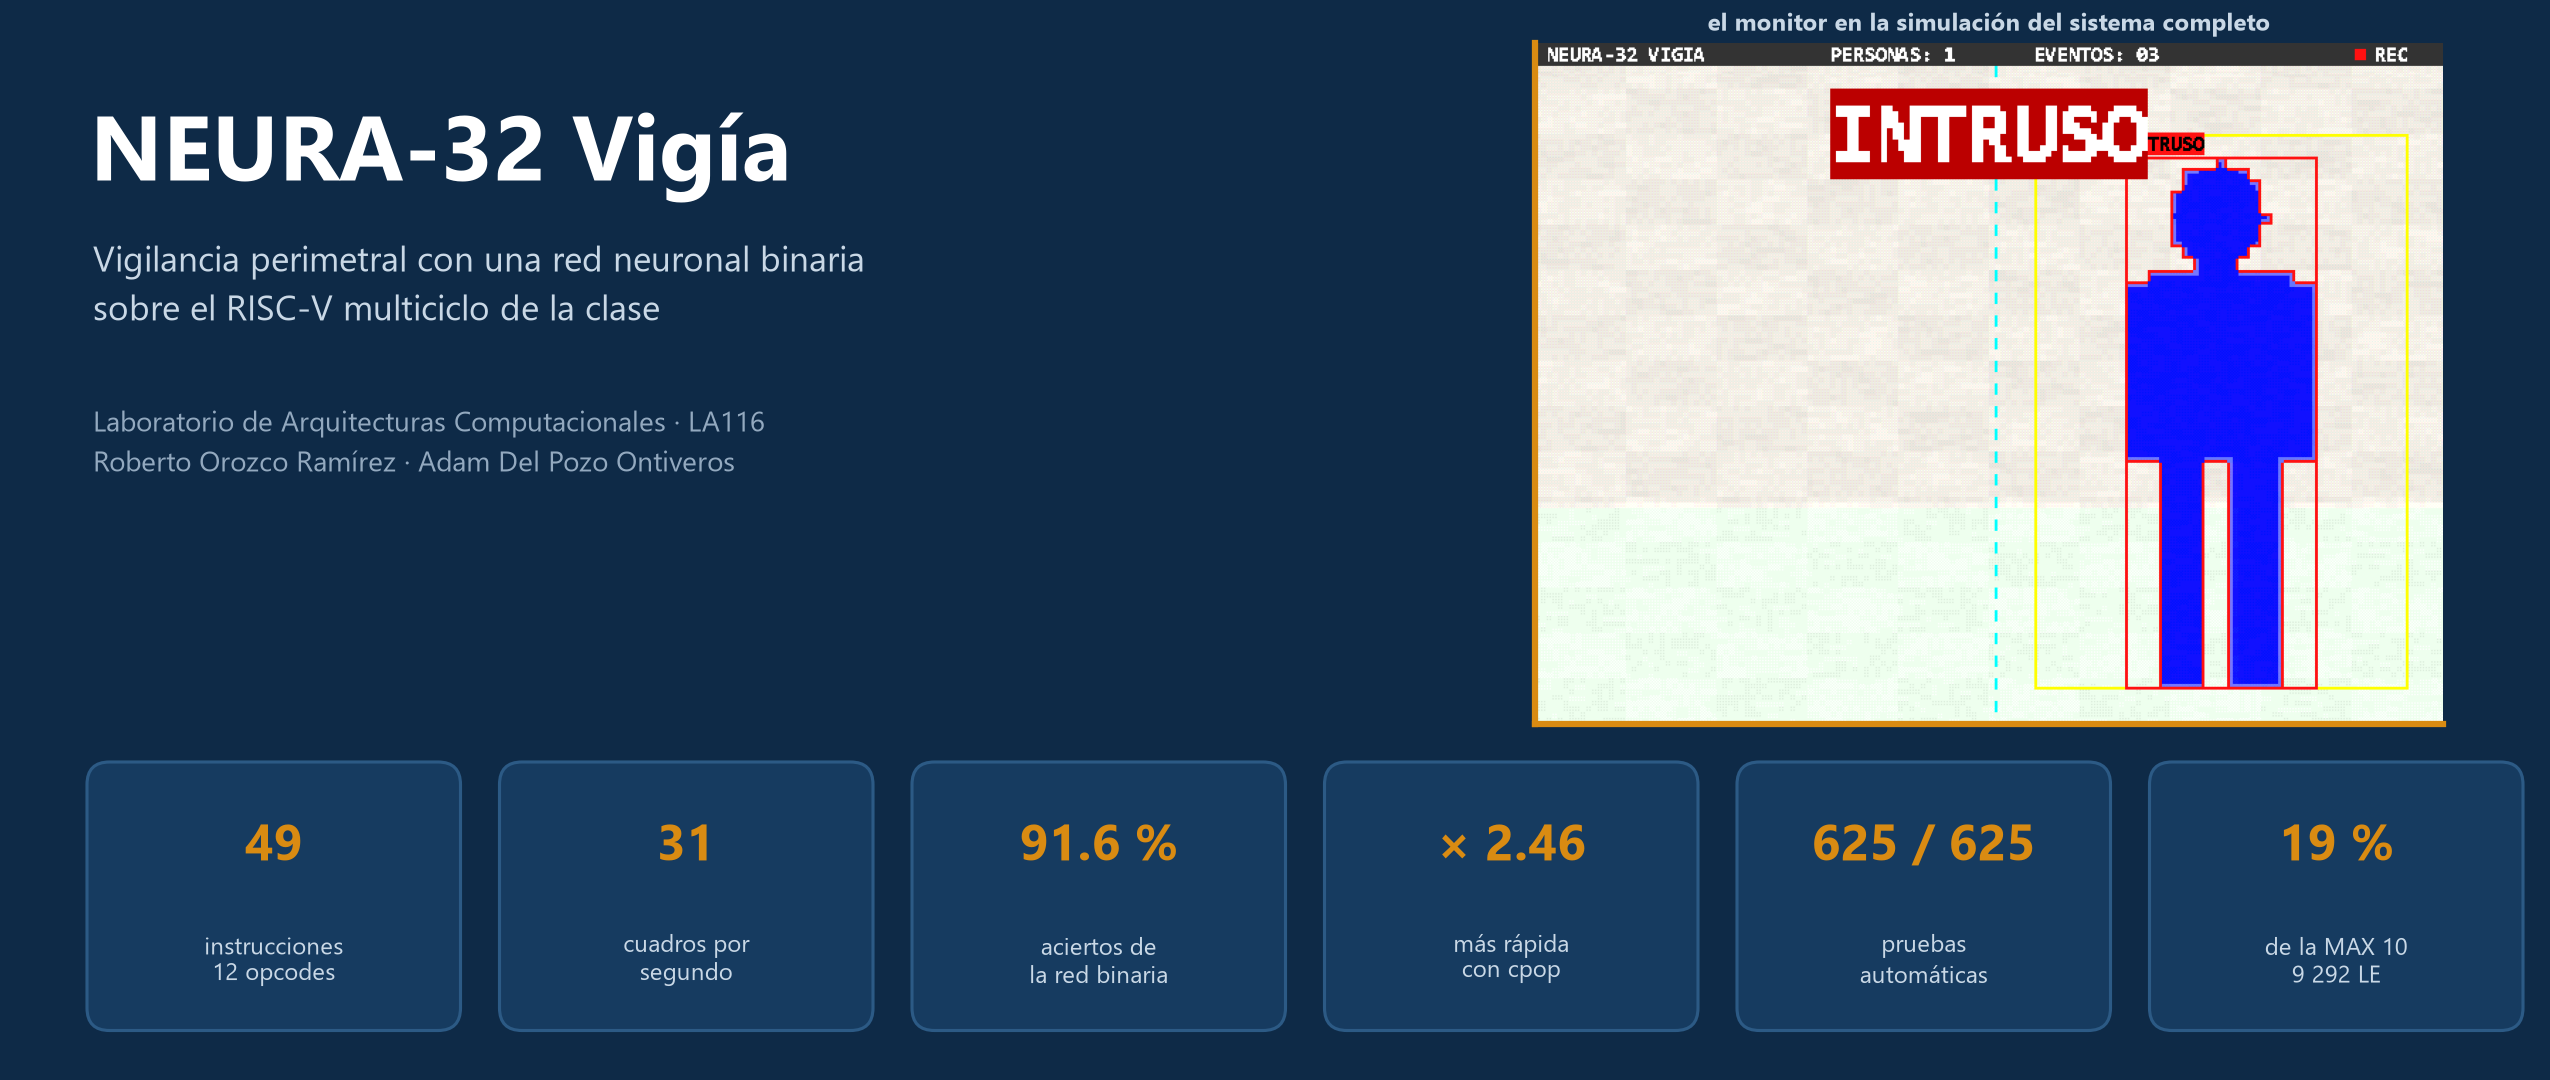
\includegraphics[width=\textwidth]{portada.png}\par
\vspace{0.8cm}
{\large
\begin{tabular}{c}
\textbf{Roberto Orozco Ramírez}\quad 184595\\[3pt]
\textbf{Adam Del Pozo Ontiveros}\quad 185611
\end{tabular}}\par
\vspace{0.9cm}
{\large San Andrés Cholula, Puebla, México\\[3pt] 27 de noviembre de 2026}\par
\vfill
{\small\color{Secondary}\href{\repo}{\nolinkurl{\repo}}}\par
\vspace{0.3cm}
{\color{Primary}\rule{\textwidth}{2.2pt}}
\end{titlepage}
\twocolumn
\setcounter{page}{1}}

\begin{document}
\hypersetup{pageanchor=false}
\portada
\hypersetup{pageanchor=true}
\selectlanguage{spanish}

\title{NEURA-32 Vigía: vigilancia perimetral con una red neuronal binaria sobre el RISC-V multiciclo de la clase}

\author{\IEEEauthorblockN{Roberto Orozco Ramírez y Adam Del Pozo Ontiveros}
\IEEEauthorblockA{Laboratorio de Arquitecturas Computacionales\\
Universidad de las Américas Puebla, San Andrés Cholula, Puebla, México}}

\maketitle
\thispagestyle{plain}
\pagestyle{plain}

\begin{abstract}
Las cámaras de vigilancia baratas avisan cada vez que algo se mueve, y casi siempre es una sombra, un cambio de luz o un animal.
En este trabajo tomamos el procesador RISC-V multiciclo que armamos en clase, el que solo calculaba $(a+b)\cdot c$, y lo
ampliamos por etapas hasta que pudo correr un programa de vigilancia completo en una DE10-Lite con una cámara OV7670. El
procesador conserva el formato de instrucciones, los bloques y la máquina de Moore de la base; lo que crece es la ALU, que
ahora tiene tres tablas de ocho operaciones elegidas por el \emph{opcode}, sin alargar \sig{funct3}. Con 49 instrucciones y
11 estados ejecuta un programa de 1\,470 instrucciones que etiqueta las siluetas que entrega la visión en hardware, las
clasifica con una red neuronal binaria de 512 entradas y 64 neuronas, y aplica reglas de zona y de cruce de línea solo a
personas confirmadas. Las instrucciones \sig{xnor} y \sig{cpop} hacen la red 2.46 veces más rápida, y el peor cuadro con una
persona ocupa el 31~\% del tiempo entre dos cuadros de la cámara. La red acierta el 91.6~\% de 1\,800 siluetas con aritmética
entera. Siete bancos de pruebas autoverificados pasan 625 de 625 comprobaciones, y el diseño ocupa 9\,292 elementos lógicos
y cierra tiempos a 33.57~MHz con un reloj de 25~MHz.
\end{abstract}

\begin{IEEEkeywords}
RISC-V, procesador multiciclo, FPGA, red neuronal binaria, \emph{popcount}, visión en hardware, vigilancia perimetral.
\end{IEEEkeywords}

\begin{otherlanguage}{english}
\renewcommand{\abstractname}{Abstract}
\begin{abstract}
Low-cost security cameras raise an alarm whenever something moves, and most of the time it is a shadow, a lighting change or
an animal. We took the multicycle RISC-V processor built in class, which only computed $(a+b)\cdot c$, and extended it in stages
until it ran a complete perimeter-surveillance program on a DE10-Lite board with an OV7670 camera. The processor keeps the
instruction format, the blocks and the Moore control unit of the original design; what grows is the ALU, which now holds three
tables of eight operations selected by the opcode, without widening \texttt{funct3}. With 49 instructions and 11 states it runs a
1,470-instruction program that labels the silhouettes produced by the hardware vision pipeline, classifies them with a binary
neural network of 512 inputs and 64 neurons, and applies zone and line-crossing rules only to confirmed people. The \texttt{xnor}
and \texttt{cpop} instructions make the network 2.46 times faster, and the worst frame with a person uses 31\% of the time
between camera frames. The network is 91.6\% accurate on 1,800 silhouettes using integer arithmetic. Seven self-checking
testbenches pass 625 of 625 checks, and the design uses 9,292 logic elements and meets timing at 33.57~MHz for a 25~MHz clock.
\end{abstract}
\end{otherlanguage}

% ---------------------------------------------------------------------------------------------
\section{Introducción}

Una cámara que manda una alerta cada vez que cambia algo en la imagen termina ignorada. El viento mueve una planta, pasa un gato
o se nubla, y el guardia deja de mirar las alertas. Los equipos comerciales de gama alta resuelven esto con un clasificador
que decide si lo que se mueve es una persona antes de avisar, y con reglas como ``entró a la zona prohibida'' o ``cruzó la línea
en el sentido contrario''. Esa lógica suele correr en un procesador de aplicaciones con una red convolucional y millones de
operaciones de punto flotante por cuadro.

Nos preguntamos si cabía en algo mucho más chico: el procesador que hicimos en clase. Era un RISC-V multiciclo de dos
instrucciones (\sig{add} y \sig{mul}) que calculaba $(a+b)\cdot c$ con un archivo de texto en hexadecimal como programa. No podía
saltar, cargar constantes ni hablar con el exterior. El reto fue hacerlo crecer sin convertirlo en otro procesador: mismo
formato de instrucción, mismos bloques con los mismos nombres y la misma unidad de control de Moore.

Las aportaciones de este trabajo son cuatro. Primero, una forma de pasar de 8 a 24 operaciones de ALU sin tocar el ancho de
\sig{funct3}, repartiéndolas en varios \emph{opcodes} del mismo tipo (sección~\ref{sec:arq}). Segundo, una división del trabajo
en la que todo lo que se repite por pixel es hardware y todo lo que decide es programa (sección~\ref{sec:vision}). Tercero, una
red neuronal binaria que el procesador evalúa con dos instrucciones nuevas, \sig{xnor} y \sig{cpop}, y que distingue personas
de cuerpo completo, de medio cuerpo y de busto (sección~\ref{sec:prog}). Cuarto, la verificación del sistema completo con un
modelo de la cámara y las mediciones en la placa (secciones~\ref{sec:verif} y~\ref{sec:res}). La Fig.~\ref{fig:resultado}
resume lo que hace el sistema.

\begin{figure}[!t]
\centering
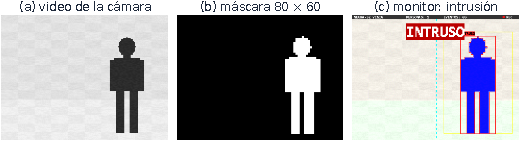
\includegraphics[width=\columnwidth]{resultado.pdf}
\caption{Un cuadro del sistema completo en simulación: (a) video de la cámara, (b) máscara de movimiento de $80\times60$ que
entrega el hardware y (c) lo que dibuja el procesador cuando confirma a una persona dentro de la zona.}
\label{fig:resultado}
\end{figure}

% ---------------------------------------------------------------------------------------------
\section{Trabajo relacionado}

Las redes neuronales binarias restringen pesos y activaciones a $\pm1$, de modo que el producto punto se reduce a un
\sig{xnor} y una cuenta de bits en~1~\cite{rastegari2016}. FINN mostró que en FPGA esa operación se mapea a lógica muy barata y
alcanza millones de clasificaciones por segundo~\cite{umuroglu2017}; ahí la red es un acelerador dedicado. Nosotros hacemos lo
contrario: la red corre como programa en un procesador de propósito general y lo único que agregamos al hardware son dos
instrucciones. La extensión de manipulación de bits de RISC-V incluye una instrucción \sig{cpop} equivalente~\cite{riscvb}, que
aquí implementamos dentro de una tabla propia.

La separación de fondo en FPGA es un tema estudiado; el modelo de Horprasert, por ejemplo, ya corre en tiempo real en
hardware~\cite{rodriguez2012}. Nuestra versión es más simple, un promedio exponencial con corrimientos sobre una rejilla de
$80\times60$, pero agrega dos detalles que hicieron falta en la placa: el fondo aprende más lento donde hay una silueta y la
máscara se escribe en dos bancos. El procesador base sigue la organización multiciclo de Patterson y
Hennessy~\cite{patterson2020} y el formato del manual de RISC-V~\cite{riscv}.

% ---------------------------------------------------------------------------------------------
\section{Arquitectura del procesador}
\label{sec:arq}

\subsection{Reglas que nos pusimos}

Partimos de \sig{riscv\_ab\_c} y sus archivos sin cambios (\sig{uc\_simple}, \sig{alu\_riscv}, \sig{decoder}, \sig{regfile},
\sig{pipo\_register}, \sig{rom} y \sig{ram}). Seis reglas guiaron todo el crecimiento: (1) las instrucciones miden 32 bits y los
campos no se mueven; (2) \sig{funct3} mide 3 bits y es directamente la operación de la ALU, \sig{alu\_op = funct3}; (3) para
tener más de ocho operaciones se agregan \emph{opcodes} del mismo tipo, no se alarga \sig{funct3}; (4) se usan los mismos bloques
y nombres de la base, con reinicio asíncrono activo en bajo; (5) los programas siguen siendo un \sig{.txt} en hexadecimal leído con
\sig{\$readmemh}, y (6) solo existe lo que algún programa del proyecto usa. La regla~(6) fue la más útil: cada instrucción nueva
tuvo que justificarse con un programa que la necesitara.

\subsection{Diez etapas}

El procesador creció en diez etapas, cada una con su banco de pruebas. La etapa~0 comprueba que el programa de la clase corre
sin cambiarle un bit. La 1 hace que la ALU decida con el \emph{opcode} y el \sig{funct3}. La 2 agrega la segunda tabla
(\sig{sub}, \sig{slt}, \sig{sltu}, \sig{sra}, \sig{xnor}, \sig{min}, \sig{minu}, \sig{max}). La 3 agrega los inmediatos S, B, U
y J, los saltos y las subrutinas. La 4 agrega los registros \sig{ALUOUT} y \sig{MDR} y la memoria por bytes. La 5 agrega la
tercera tabla con el divisor, \sig{cpop}, \sig{abs}, \sig{sgt} y \sig{clamp}. La 6 agrega entradas y salidas mapeadas en
memoria y \sig{ecall}; la 7, un cargador de programas por JTAG; la 8, la visión, y la 9, el programa de vigilancia.

\subsection{Repertorio de instrucciones}

La Tabla~\ref{tab:isa} muestra la idea central. El \emph{opcode} escoge una tabla de ocho operaciones y \sig{funct3} escoge la
operación dentro de ella. \sig{OP\_R1} es exactamente la tabla de la clase, por eso \sig{programa\_ab\_c.txt} corre igual. En total
son 49 instrucciones con 12 \emph{opcodes}. El \sig{funct7} conserva sus siete bits en el formato, pero el procesador ya no lo
necesita para decidir. Dentro de la ALU esto queda como un \sig{case} del \emph{opcode} con un \sig{case} de ocho operaciones
adentro, y agregar una operación es agregar un renglón.

\begin{table}[!t]
\centering
\caption{Las tres tablas de la ALU y la de saltos. El \emph{opcode} elige la columna y \sig{funct3} el renglón.}
\label{tab:isa}
\tabfont
\setlength{\tabcolsep}{4.2pt}
\begin{tabular}{@{}cllll@{}}
\toprule
\sig{funct3} & \sig{OP\_R1}/\sig{OP\_I1} & \sig{OP\_R2}/\sig{OP\_I2} & \sig{OP\_R3} & \sig{OP\_BRANCH} \\
 & (la de la clase) & & & \\
\midrule
000 & \sig{add} & \sig{sub}  & \sig{divu}  & \sig{beq} \\
001 & \sig{mul} & \sig{slt}  & \sig{remu}  & \sig{bne} \\
010 & \sig{and} & \sig{sltu} & \sig{cpop}  & -- \\
011 & \sig{or}  & \sig{sra}  & \sig{abs}   & -- \\
100 & \sig{xor} & \sig{xnor} & \sig{sgt}   & \sig{blt} \\
101 & \sig{nota}& \sig{min}  & \sig{clamp} & \sig{bge} \\
110 & \sig{sll} & \sig{minu} & --          & \sig{bltu} \\
111 & \sig{srl} & \sig{max}  & --          & \sig{bgeu} \\
\bottomrule
\end{tabular}
\end{table}

\subsection{Camino de datos y unidad de control}

La Fig.~\ref{fig:ruta} muestra el camino de datos final. Se conservan \sig{PC}, \sig{IMEM}, \sig{IR}, \sig{DEC}, \sig{RF},
\sig{ALU} y \sig{DMEM}, y se agregan cuatro registros. \sig{PCI} guarda el PC de la instrucción en curso, porque cuando la
instrucción llega a \sig{IR} el PC ya avanzó y el destino de un salto se calcula desde el PC viejo. \sig{ALUOUT} y \sig{MDR}
guardan el resultado y el dato leído para que la escritura al banco use valores estables. La memoria de datos son cuatro
\sig{ram} de 8 bits de la clase, una por byte, lo que permite \sig{sb} y \sig{sh} y deja que Quartus las ponga en bloques M9K. El
divisor resta y corre un bit por ciclo, porque una división de 32 bits no cabe en un periodo de 40~ns.

\begin{figure*}[!t]
\centering
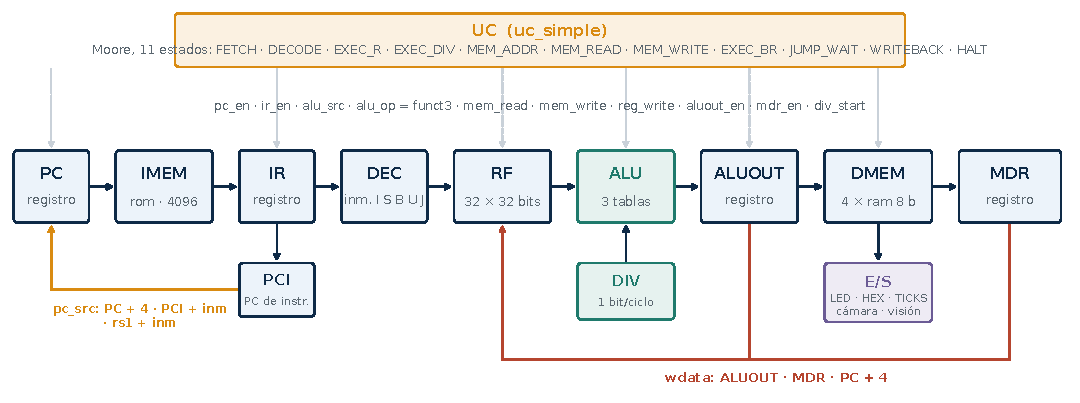
\includegraphics[width=\textwidth]{ruta_datos.pdf}
\caption{Camino de datos de NEURA-32. En azul, los bloques de la clase; en verde, la ALU de tres tablas y el divisor; en morado,
las entradas y salidas. Las dos rutas de regreso son \sig{pc\_src} hacia el PC y \sig{wdata} hacia el banco de registros.}
\label{fig:ruta}
\end{figure*}

La unidad de control sigue siendo una máquina de Moore: sus salidas dependen solo del estado y de la instrucción en \sig{IR}.
Pasó de los estados de la base a 11 (Fig.~\ref{fig:uc}). Las instrucciones aritméticas tardan 4 ciclos, las cargas 5, un salto
que no se cumple 3 y uno que se cumple 4, porque \sig{JUMP\_WAIT} deja un ciclo para que la memoria de programa lea el destino.
\sig{divu} y \sig{remu} esperan en \sig{EXEC\_DIV} los 32 ciclos del divisor y tardan 36. La Fig.~\ref{fig:fsm} muestra la misma
máquina tal como la reconoce Quartus después de la síntesis, con su tabla de transiciones.

\begin{figure}[!t]
\centering
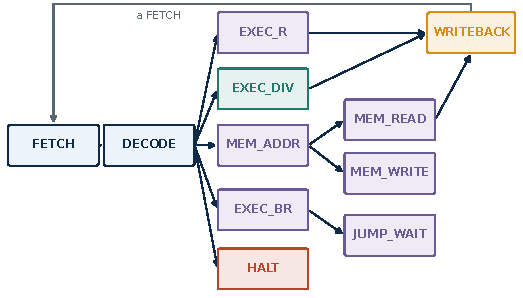
\includegraphics[width=\columnwidth]{uc.pdf}
\caption{Estados de \sig{uc\_simple}. Desde \sig{DECODE} cada tipo de instrucción toma su camino y todas regresan a
\sig{FETCH}; \sig{ecall} termina en \sig{HALT}.}
\label{fig:uc}
\end{figure}

\begin{figure}[!t]
\centering
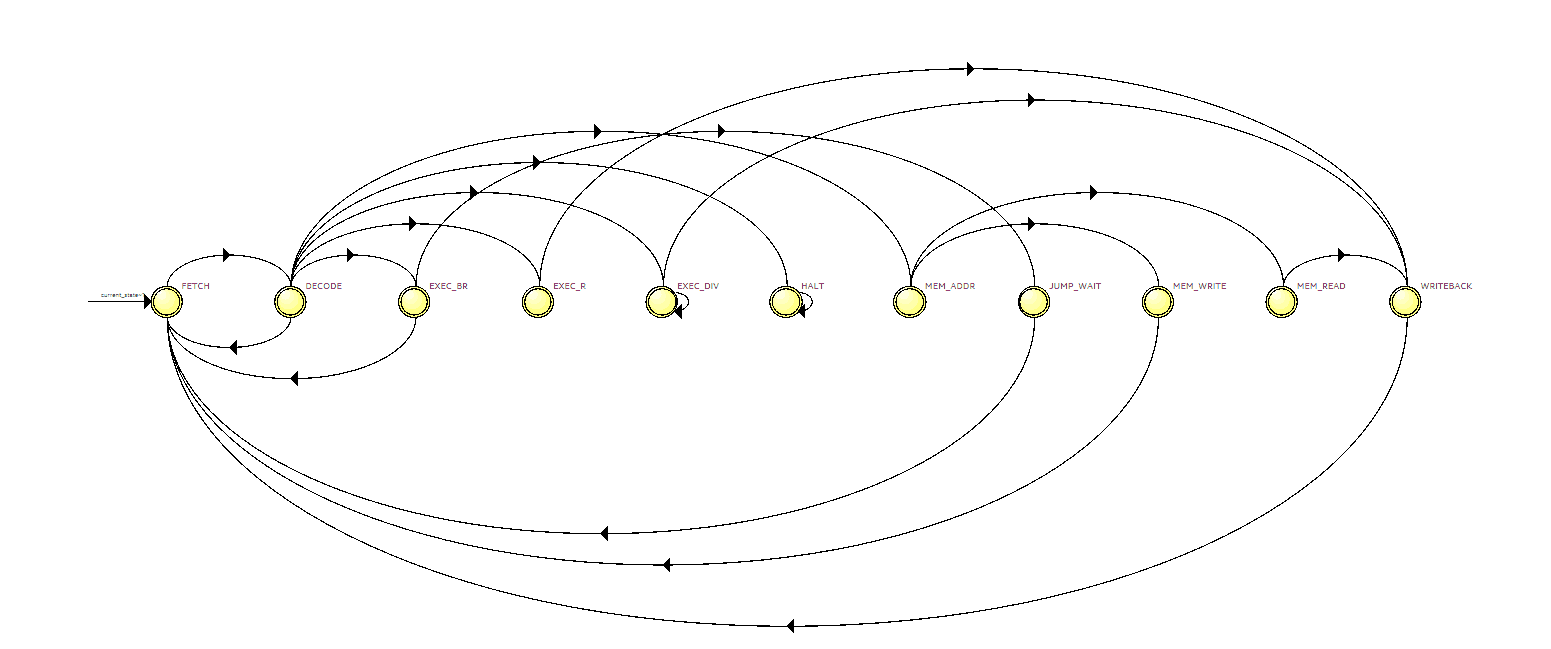
\includegraphics[width=\columnwidth]{rtl_uc_simple_estados.png}
\caption{La unidad de control en el \emph{State Machine Viewer} de Quartus: los 11 estados de \sig{current\_state} y, abajo, las
transiciones con su condición.}
\label{fig:fsm}
\end{figure}

\subsection{Los bloques después de la síntesis}

Para revisar que la síntesis respetara la jerarquía exportamos el RTL Viewer de cada bloque. En la Fig.~\ref{fig:soc} se ve el
sistema completo, con el procesador, la visión, los periféricos, el cargador y los registros que el programa usa para dibujar.
La Fig.~\ref{fig:cpop} es un acercamiento a la ALU: \sig{cpop} quedó como un árbol de sumadores que junta los bits de dos en dos,
luego de cuatro en cuatro, hasta una cuenta de 0 a 32 en 9 bits. Ese árbol es la razón de la aceleración de la red.

\begin{figure*}[!t]
\centering
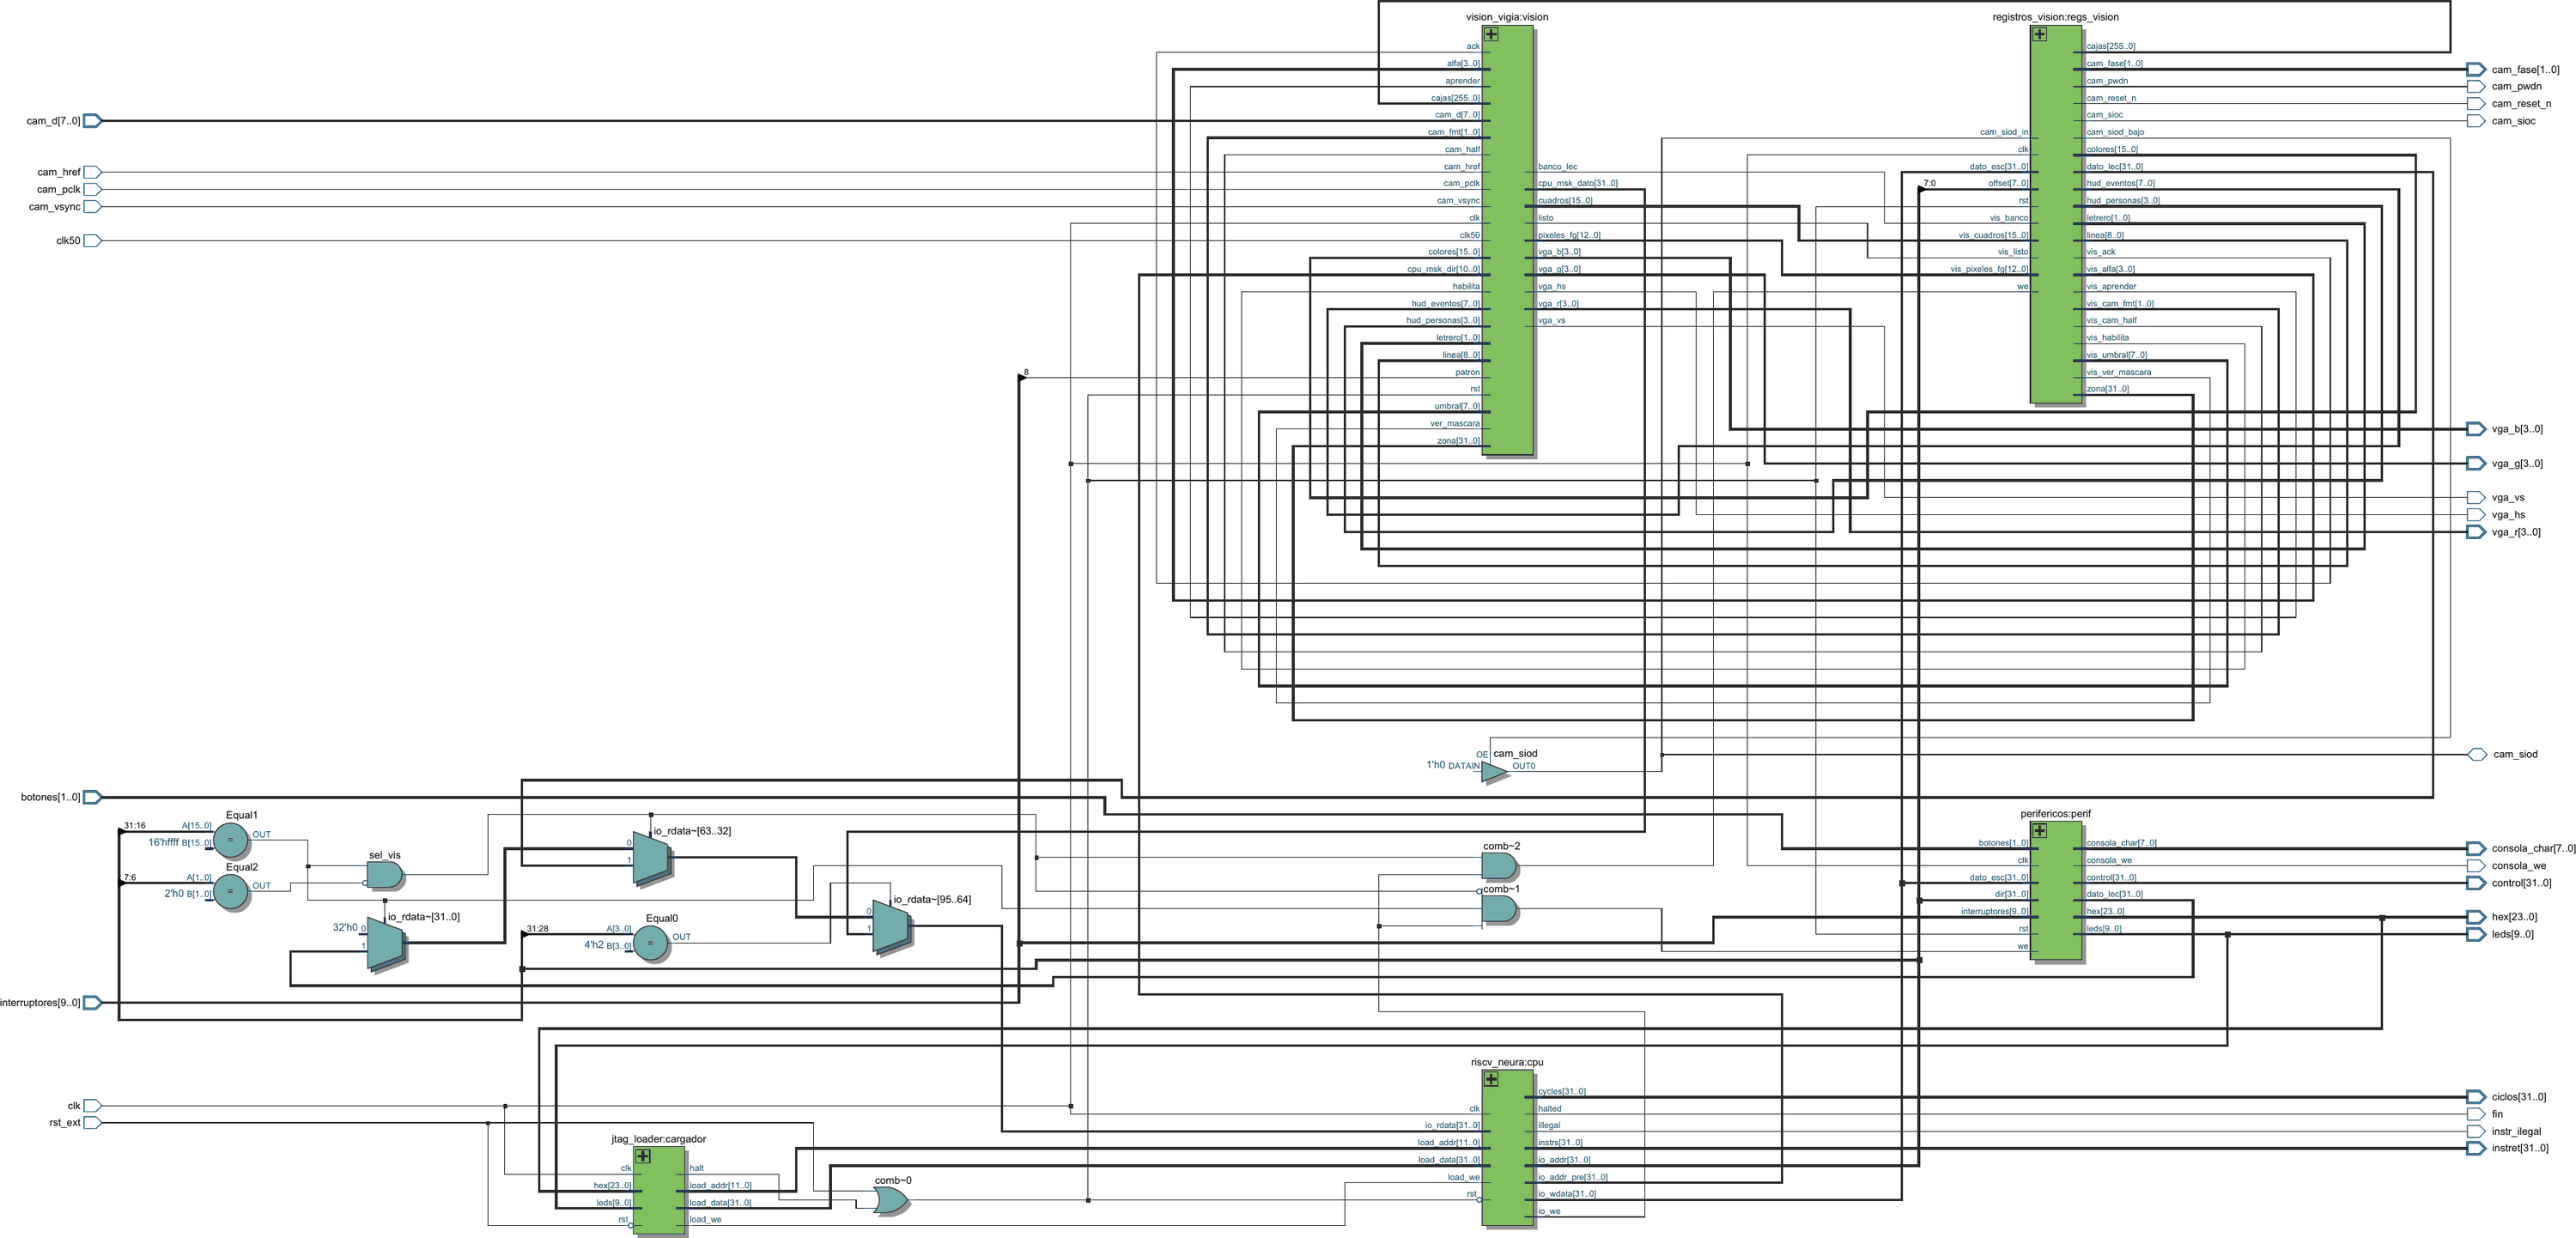
\includegraphics[width=0.84\textwidth]{rtl_soc_neura32.png}
\caption{El sistema completo, \sig{soc\_neura32}, en el RTL Viewer de Quartus: el procesador (\sig{cpu}), la visión, los
registros de dibujo, los periféricos y el cargador por JTAG, unidos por el bus de entradas y salidas.}
\label{fig:soc}
\end{figure*}

\begin{figure}[!t]
\centering
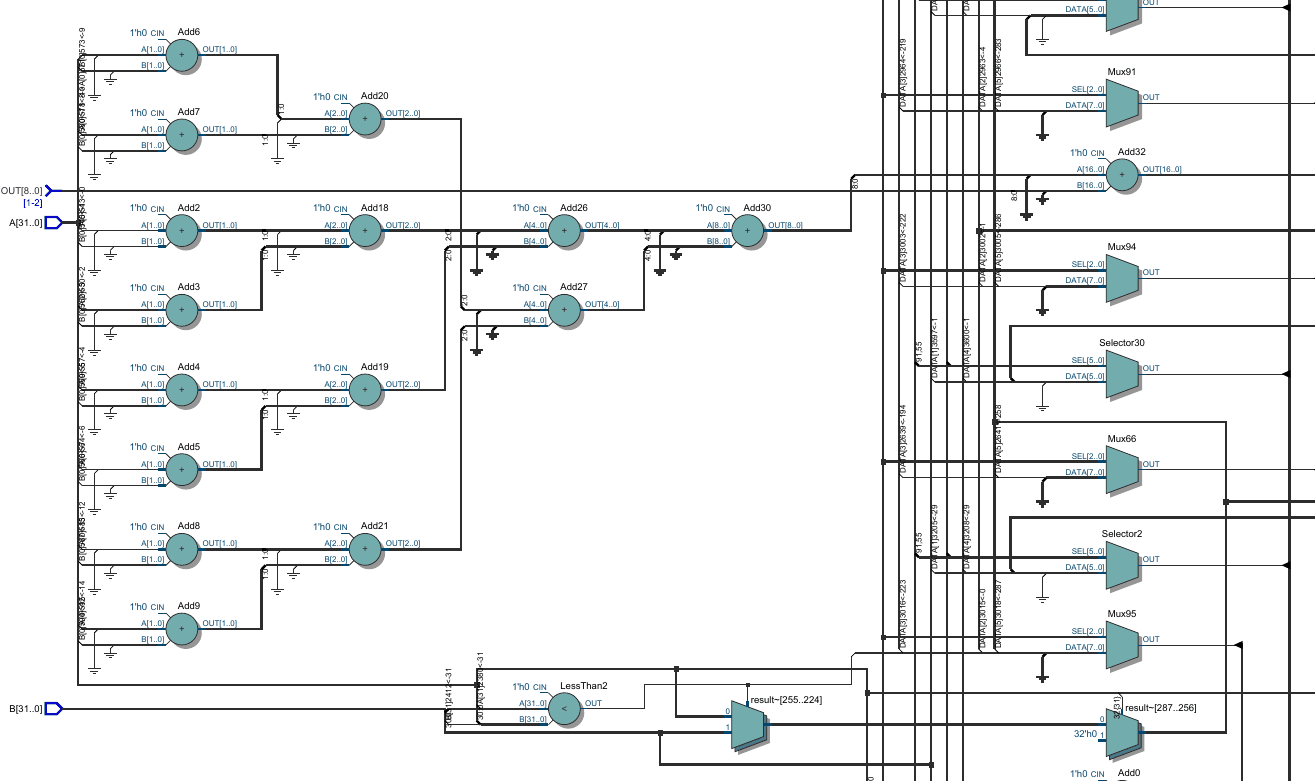
\includegraphics[width=\columnwidth]{rtl_alu_cpop.png}
\caption{Acercamiento a \sig{alu\_riscv} en el RTL Viewer: el árbol de sumas de \sig{cpop} (\sig{Add2}\ldots\sig{Add30}) y, abajo,
el comparador de \sig{slt}.}
\label{fig:cpop}
\end{figure}

\subsection{Programas y cargador}

Los programas se escriben en Verilog con funciones que arman cada instrucción bit a bit según su formato (\sig{ADD(rd,rs1,rs2)},
\sig{LW(rd,rs1,inm)}, \sig{CPOP(\ldots)}). Un generador de dos pasadas resuelve las etiquetas y escribe el \sig{.txt} que lee la
memoria de programa. Con la placa ya grabada, un \emph{script} de Tcl detiene el procesador, escribe otro \sig{.txt} por el cable
USB-Blaster y lo suelta en la dirección~0, sin volver a compilar. Así probamos en la misma placa el programa de la clase, un
Fibonacci, la prueba de todas las instrucciones, un clasificador de $3\times3$ y la vigilancia.

% ---------------------------------------------------------------------------------------------
\section{Visión en hardware}
\label{sec:vision}

Un procesador que tarda cuatro ciclos por instrucción no puede tocar cada pixel de un video de $320\times240$ a 31 cuadros por
segundo. Por eso todo lo que se repite por pixel es hardware, sin procesador (Fig.~\ref{fig:vision}). La FPGA le da a la cámara
un reloj de 25~MHz, y el programa la configura por SCCB~\cite{ov7670} a $320\times240$ en YUV 4:2:2. \sig{cam\_capture} muestrea las señales de
la cámara con el reloj de 50~MHz a través de dos flip-flops, de modo que no hay cruces de reloj sin sincronizar, y filtra pulsos
falsos: \sig{VSYNC} cuenta solo si dura más de 5~µs y un renglón termina solo tras 300~ns de \sig{HREF} en bajo.

\begin{figure*}[!t]
\centering
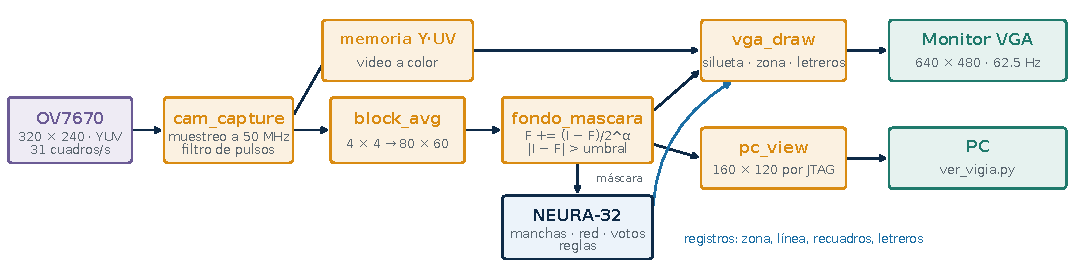
\includegraphics[width=\textwidth]{vision.pdf}
\caption{La visión. Todo lo que se repite por pixel es hardware; NEURA-32 solo lee la máscara y escribe en los registros lo que
se dibuja encima del video.}
\label{fig:vision}
\end{figure*}

\sig{block\_avg} promedia bloques de $4\times4$ pixeles y entrega una rejilla de $80\times60$ con menos ruido. \sig{fondo\_mascara}
guarda un fondo $F$ por celda y lo actualiza con un promedio exponencial que solo necesita corrimientos:
\begin{equation}
F \leftarrow F + \frac{I - F}{2^{\alpha}}, \qquad m = \bigl[\,|I - F| > u\,\bigr],
\label{eq:fondo}
\end{equation}
donde $I$ es el brillo actual, $u$ el umbral que se elige con tres interruptores y $m$ el bit de la máscara. Donde hay una
silueta el fondo aprende cuatro veces más lento, para que una persona quieta no se borre. La máscara se escribe en dos bancos:
la cámara llena uno mientras el procesador lee el otro.

El monitor trabaja a $640\times480$ y 62.5~Hz, exactamente dos cuadros por cada cuadro de la cámara, y su barrido se engancha a
ella: el renglón 0 se escribe cuando el monitor va en su renglón 16, así que nunca lee el renglón que se está escribiendo y no hay
cortes aunque la cámara se mueva. \sig{vga\_draw} convierte YUV a RGB con sumas y corrimientos, suaviza la ampliación con el
renglón anterior guardado en una M9K y dibuja encima la zona, la línea, hasta ocho recuadros con letrero y la barra de estado.
Cuando no hay monitor, \sig{pc\_view} manda el mismo video a la computadora por JTAG.

% ---------------------------------------------------------------------------------------------
\section{El programa de vigilancia}
\label{sec:prog}

\subsection{Flujo por cuadro}

El programa tiene 1\,470 instrucciones más 1\,466 palabras de tablas y pesos. Al arrancar reinicia la cámara, lee su
identificación (PID 0x76, VER 0x73), le escribe su tabla de registros por SCCB hecho por software, hace una autoprueba de la red
y, a los dos segundos, fija la exposición y aprende el fondo vacío. Después, 31 veces por segundo: (1) etiqueta las manchas de
la máscara con relleno por inundación y una pila en RAM, y saca el recuadro de cada una con \sig{min} y \sig{max}; (2) recorta
cada mancha a $16\times32$ bits con acumuladores, sin dividir; (3) la clasifica con la red; (4) la empareja con su pista por
distancia Manhattan (\sig{abs}) y suma o resta un voto, y (5) si la pista llega a dos votos, la persona queda confirmada y se le
aplican las reglas. Cruzar la línea cuenta una entrada o una salida, y en el sentido prohibido es alarma; tener los pies tres
cuadros seguidos dentro de la zona también. Si cambia más de la mitad de la imagen tres cuadros seguidos, el programa supone que
movieron la cámara o cambió la luz, olvida las pistas y vuelve a aprender el fondo sin dar alarma.

\subsection{Red neuronal binaria}

La entrada son los 512 bits del recorte, guardados en 16 palabras. La capa oculta tiene 64 neuronas con pesos de un bit:
\begin{equation}
a_j = \Bigl[\,\textstyle\sum_{i=1}^{16} \mathrm{cpop}\bigl(\mathrm{xnor}(x_i, w_{j,i})\bigr) \ge T_j\,\Bigr],
\label{eq:oculta}
\end{equation}
y la salida tiene tres clases con pesos de 8 bits, $o_k = B_k + \sum_j W_{k,j}\,a_j$, donde gana la mayor (\sig{sgt}). Cada
palabra cuesta cinco instrucciones con \sig{xnor} y \sig{cpop}, contra 17 si los bits se cuentan con corrimientos, máscaras y
sumas. La red se entrenó fuera del procesador con 12\,000 siluetas sintéticas en la misma rejilla y con la misma aritmética entera
del programa, incluyendo los defectos de una máscara real (bordes comidos, huecos y sombra en los pies). Las personas aparecen de
cuerpo completo, de medio cuerpo y de busto, porque cerca de la cámara el borde de la imagen las corta.

\begin{figure}[!t]
\centering
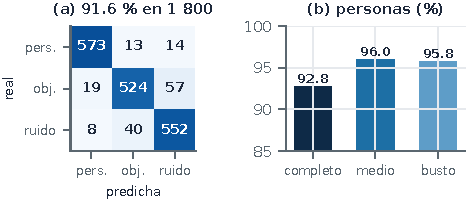
\includegraphics[width=\columnwidth]{red.pdf}
\caption{(a) Matriz de confusión de la red con aritmética entera sobre 1\,800 siluetas de prueba. (b) Personas reconocidas en 400
siluetas nuevas de cada tipo.}
\label{fig:red}
\end{figure}

Con aritmética entera, que es lo que ejecuta el procesador, la red acierta el 91.6~\% de 1\,800 siluetas de prueba
(Fig.~\ref{fig:red}a). El error más común es confundir un objeto con ruido (57 casos), que no dispara alarmas; solo 13 personas
se toman por objeto. Por tipo de persona reconoce el 92.8~\% de cuerpo completo, el 96.0~\% de medio cuerpo y el 95.8~\% de busto
(Fig.~\ref{fig:red}b). El voto entre cuadros absorbe los errores aislados, de modo que un cuadro mal clasificado no hace
parpadear el letrero.

% ---------------------------------------------------------------------------------------------
\section{Verificación}
\label{sec:verif}

Todo se simula con Icarus Verilog y compila sin errores ni advertencias en Active-HDL. Cada banco se revisa solo y termina con
\sig{PRUEBAS: n ERRORES: 0} (Tabla~\ref{tab:verif}). El más importante es \sig{tb\_vigia}, que corre el programa completo con un
modelo de la OV7670: responde por SCCB, genera \sig{PCLK} con la fórmula que medimos en la cámara real y produce una escena a
color con textura y ruido. El guion mueve la cámara, hace cruzar a un perro por la zona y después mete a una persona que cruza la
línea en el sentido prohibido y se queda. El programa vuelve a aprender el fondo sin alarmas, clasifica al perro como no persona,
cuenta una entrada y marca los dos motivos de intrusión. Las puntuaciones de la red calculadas por el procesador coinciden con
las de un modelo de referencia en Verilog.

\begin{table}[!t]
\centering
\caption{Bancos de pruebas autoverificados.}
\label{tab:verif}
\tabfont
\setlength{\tabcolsep}{3.5pt}
\begin{tabularx}{\columnwidth}{@{}lXr@{}}
\toprule
Banco & Qué comprueba & Pasan \\
\midrule
\sig{tb\_programa\_ab\_c} & el programa de la clase sin cambios & 3/3 \\
\sig{tb\_uc\_simple} & recorrido y señales de cada estado & 28/28 \\
\sig{tb\_prueba\_isa} & las 49 instrucciones, saltos y bytes & 64/64 \\
\sig{tb\_red\_neuronal} & clasificador $3\times3$ contra referencia & 481/481 \\
\sig{tb\_cargador} & carga de programa por JTAG en marcha & 7/7 \\
\sig{tb\_vision} & color, máscara, monitor y vista en PC & 11/11 \\
\sig{tb\_vigia} & sistema completo con cámara simulada & 31/31 \\
\midrule
\multicolumn{2}{@{}l}{Total} & 625/625 \\
\bottomrule
\end{tabularx}
\end{table}

En la placa comprobamos el cableado de las 16 señales, la respuesta por SCCB, la relación entre \sig{XCLK} y \sig{PCLK}, la
ventana de imagen y la fase de reloj. La Fig.~\ref{fig:placa} muestra capturas reales leídas por JTAG: con \sig{XCLK} sin invertir
se rompen los renglones y con \sig{XCLK} a $180^\circ$ la imagen sale limpia; los 157 registros de ajuste quitan las rayas del
sensor. Con el diseño completo grabado en la memoria flash, la cámara entregó 31 cuadros por segundo y el monitor se mantuvo
enganchado, sin cortes al mover la cámara.

\begin{figure*}[!t]
\centering
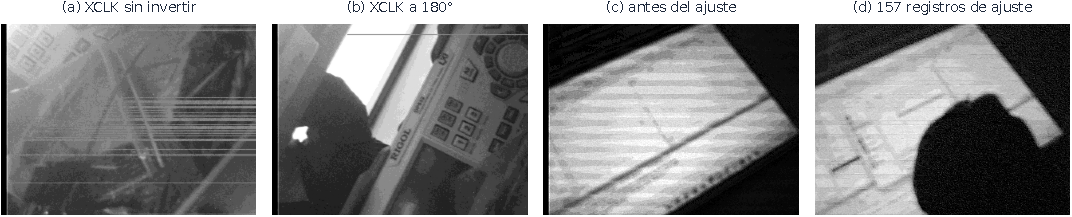
\includegraphics[width=\textwidth]{placa.pdf}
\caption{Capturas reales de la OV7670 en la DE10-Lite, leídas por JTAG: (a) y (b) efecto de la fase de \sig{XCLK}; (c) y (d)
la misma escena antes y después de escribir los 157 registros de ajuste.}
\label{fig:placa}
\end{figure*}

% ---------------------------------------------------------------------------------------------
\section{Resultados}
\label{sec:res}

\subsection{Rendimiento}

La Fig.~\ref{fig:rend} resume las mediciones. Los ciclos por instrucción van de 4.00 en el programa de la clase a 4.66 en la
prueba del repertorio, que incluye divisiones de 36 ciclos; el programa de vigilancia completo ejecutó 5\,558\,959 instrucciones
en 23\,483\,842 ciclos, un CPI de 4.22. Una clasificación tarda 82\,859 ciclos contando los bits por software y 33\,678 con
\sig{xnor} y \sig{cpop}, 2.46 veces menos, medido por el propio programa con el contador \sig{TICKS}. La cámara entrega un cuadro
cada 32~ms, que a 25~MHz son 800\,000 ciclos. Procesar una máscara con una persona, desde el etiquetado hasta el dibujo, tomó como
máximo 251\,942 ciclos (10.1~ms), el 31~\% del tiempo disponible, y la respuesta llega en el cuadro siguiente.

\begin{figure*}[!t]
\centering
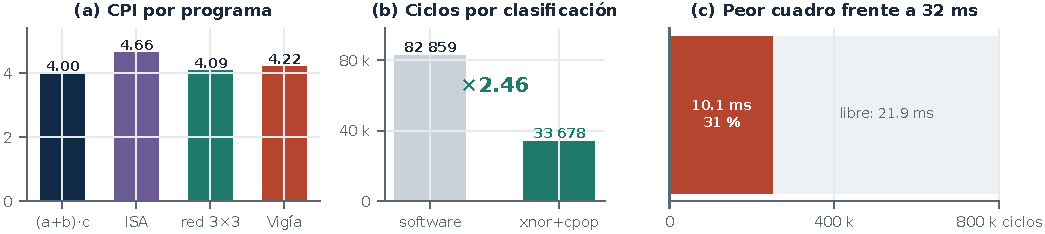
\includegraphics[width=\textwidth]{rendimiento.pdf}
\caption{(a) Ciclos por instrucción de cada programa. (b) Ciclos por clasificación de la red con y sin \sig{cpop}. (c) El peor
cuadro con una persona frente a los 32~ms entre dos cuadros de la cámara.}
\label{fig:rend}
\end{figure*}

\subsection{Recursos}

La Tabla~\ref{tab:rec} y la Fig.~\ref{fig:rec} muestran la ocupación en la MAX~10 de la DE10-Lite~\cite{de10lite} según Quartus Prime 24.1 Lite. La lógica es
moderada, el 19~\% del dispositivo, y se reparte entre el monitor, el banco de registros, el promedio de la visión y la ALU. Lo que
casi se acaba es la memoria: 164 de 182 bloques M9K, casi todo video. El reloj de 25~MHz cierra tiempos con 33.57~MHz en el modelo
lento a 85~$^\circ$C, así que queda margen.

\begin{table}[!t]
\centering
\caption{Recursos en la MAX~10 10M50DAF484C7G.}
\label{tab:rec}
\tabfont
\begin{tabular}{@{}lrr@{}}
\toprule
Recurso & Usado & Disponible \\
\midrule
Elementos lógicos & 9\,292 (19~\%) & 49\,760 \\
Registros & 4\,062 & -- \\
Bloques M9K & 164 (90~\%) & 182 \\
Bits de memoria & 1\,214\,976 (72~\%) & 1\,677\,312 \\
Multiplicadores de 9 bits & 6 & 288 \\
Pines & 121 & 360 \\
$f_{\max}$, reloj de 25~MHz & 33.57~MHz & -- \\
\bottomrule
\end{tabular}
\end{table}

\begin{figure*}[!t]
\centering
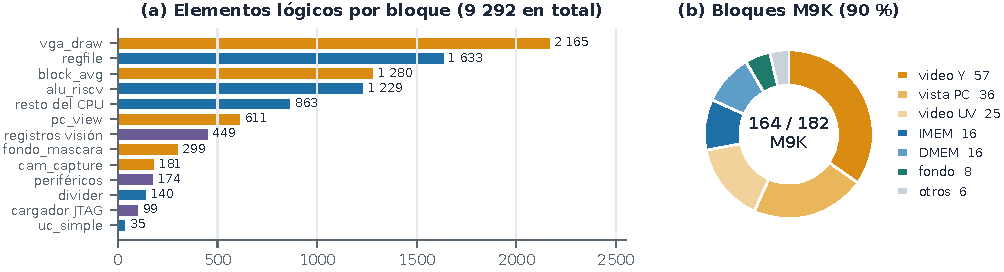
\includegraphics[width=\textwidth]{recursos.pdf}
\caption{(a) Elementos lógicos por bloque según el reporte del \emph{Fitter}. (b) Reparto de los bloques M9K: la memoria es casi
toda video.}
\label{fig:rec}
\end{figure*}

\subsection{Limitaciones}

La red se entrenó con siluetas sintéticas y el 91.6~\% se midió con ellas; todavía no tenemos una medición con escenas reales
etiquetadas. La red tampoco separa a dos personas que caminan juntas, porque salen como una sola mancha. La prueba del sistema
completo usa la cámara simulada a $160\times120$ para que no dure horas, aunque el programa y la rejilla de detección son los
mismos que en la placa. Y como el procesador sigue siendo multiciclo, el 31~\% de ocupación es con una persona; con muchas manchas
a la vez el tiempo crece.

% ---------------------------------------------------------------------------------------------
\section{Conclusiones}

El procesador de la clase alcanzó para una aplicación real sin cambiarle la forma: sigue siendo multiciclo, con los mismos bloques,
y el programa $(a+b)\cdot c$ todavía corre en él. Lo que cambió fue cuántas cosas sabe hacer cada bloque. Mantener \sig{funct3} en
tres bits y repartir las operaciones en varios \emph{opcodes} dejó una ALU fácil de leer y de ampliar. Las instrucciones nuevas se
justificaron midiendo: \sig{xnor} y \sig{cpop} hacen la red 2.46 veces más rápida, y con \sig{min}, \sig{max}, \sig{abs} y
\sig{sgt} el programa cabe en un cuadro aunque cada instrucción tarde cuatro ciclos. La decisión que lo hizo posible fue repartir
el trabajo: lo que se repite por pixel es hardware, y lo que decide es programa que se cambia cargando otro \sig{.txt}.

Como trabajo futuro queremos medir la red con video real etiquetado, entrenar un clasificador más grande que separe a varias
personas juntas, guardar la foto de cada evento en una memoria externa y resolver los saltos un ciclo antes para bajar el CPI. El
código, los bancos de pruebas y las figuras están en \url{\repo}.

% ---------------------------------------------------------------------------------------------
\balance
\begin{thebibliography}{9}
\footnotesize

\bibitem{riscv}
A.~Waterman y K.~Asanović, Eds., \emph{The RISC-V Instruction Set Manual, Volume~I: Unprivileged ISA}. RISC-V International.

\bibitem{riscvb}
RISC-V International, \emph{RISC-V Bit-Manipulation ISA-Extensions}, versión 1.0.0, 2021.

\bibitem{patterson2020}
D.~A.~Patterson y J.~L.~Hennessy, \emph{Computer Organization and Design RISC-V Edition}, 2.ª ed. Cambridge, MA, EE.~UU.:
Morgan Kaufmann, 2020.

\bibitem{rastegari2016}
M.~Rastegari, V.~Ordonez, J.~Redmon y A.~Farhadi, ``XNOR-Net: ImageNet classification using binary convolutional neural
networks'', en \emph{Proc. ECCV}, 2016, pp.~525--542.

\bibitem{umuroglu2017}
Y.~Umuroglu \emph{et al.}, ``FINN: A framework for fast, scalable binarized neural network inference'', en \emph{Proc.
ACM/SIGDA Int. Symp. Field-Programmable Gate Arrays (FPGA'17)}, 2017, pp.~65--74.

\bibitem{rodriguez2012}
M.~Rodríguez-Gómez \emph{et al.}, ``FPGA implementation for real-time background subtraction based on Horprasert model'',
\emph{Sensors}, vol.~12, núm.~1, pp.~585--611, 2012.

\bibitem{de10lite}
Terasic, \emph{DE10-Lite User Manual}, 2022.

\bibitem{ov7670}
OmniVision, \emph{OV7670/OV7171 CMOS VGA CameraChip Implementation Guide} y hoja de datos del OV7670.

\end{thebibliography}

\end{document}
